%%%%%%%%%%%%%%%%%%%%%%%%%%%%%%%%%%%%%%%%%
% Beamer Presentation
% LaTeX Template
% Version 1.0 (10/11/12)
%
% This template has been downloaded from:
% http://www.LaTeXTemplates.com
%
% License:
% CC BY-NC-SA 3.0 (http://creativecommons.org/licenses/by-nc-sa/3.0/)
%
%%%%%%%%%%%%%%%%%%%%%%%%%%%%%%%%%%%%%%%%%

%----------------------------------------------------------------------------------------
%	PACKAGES AND THEMES
%----------------------------------------------------------------------------------------

\documentclass[9pt]{beamer}
\usepackage{CJK}
\usepackage{ctex}
\usepackage{graphicx}
\usepackage{subfigure}
\usepackage{longtable}
\usepackage{rotating}
\usepackage{multirow}
\usepackage{algorithm}
\usepackage{algorithmic}
\usepackage{mathtools}
\usepackage{animate}
\usepackage{amsmath}
%\usepackage{media9}
%% A LATEX package for embedding interactive Adobe Flash (SWF) and 3D files (Adobe U3D & PRC) as well as video and sound files or streams (FLV, MP4/H.246, MP3) into PDF documents with Adobe Reader-9/X
%compatibility.
\renewcommand{\algorithmicrequire}{\textbf{Input:}}   %Use Input in the format of Algorithm
\renewcommand{\algorithmicensure}{\textbf{Output:}}  %UseOutput in the format of Algorithm
\newcommand{\e}[1]{\ensuremath{\times 10^{#1}}}
%\mode<presentation>{\usetheme{Madrid}}

\mode<presentation> {

% The Beamer class comes with a number of default slide themes
% which change the colors and layouts of slides. Below this is a list
% of all the themes, uncomment each in turn to see what they look like.

%\usetheme{default}
%\usetheme{AnnArbor}
%\usetheme{Antibes}
%\usetheme{Bergen}
%\usetheme{Berkeley}
%\usetheme{Berlin}
%\usetheme{Boadilla}
%\usetheme{CambridgeUS}
%\usetheme{Copenhagen}
%\usetheme{Darmstadt}
%\usetheme{Dresden}
%\usetheme{Frankfurt}
%\usetheme{Goettingen}
%\usetheme{Hannover}
%\usetheme{Ilmenau}
%\usetheme{JuanLesPins}
%\usetheme{Luebeck}
\usetheme{Madrid}
%\usetheme{Malmoe}
%\usetheme{Marburg}
%\usetheme{Montpellier}
%\usetheme{PaloAlto}
%\usetheme{Pittsburgh}
%\usetheme{Rochester}
%\usetheme{Singapore}
%\usetheme{Szeged}
%\usetheme{Warsaw}

% As well as themes, the Beamer class has a number of color themes
% for any slide theme. Uncomment each of these in turn to see how it
% changes the colors of your current slide theme.

%\usecolortheme{albatross}
\usecolortheme{beaver}
%\usecolortheme{beetle}
%\usecolortheme{crane}
%\usecolortheme{dolphin}
%\usecolortheme{dove}
%\usecolortheme{fly}
%\usecolortheme{lily}
%\usecolortheme{orchid}
%\usecolortheme{rose}
%\usecolortheme{seagull}
%\usecolortheme{seahorse}
%\usecolortheme{whale}
%\usecolortheme{wolverine}

%\setbeamertemplate{footline} % To remove the footer line in all slides uncomment this line
%\setbeamertemplate{footline}[page number] % To replace the footer line in all slides with a simple slide count uncomment this line

%\setbeamertemplate{navigation symbols}{} % To remove the navigation symbols from the bottom of all slides uncomment this line
}

\usepackage{graphicx} % Allows including images
\usepackage{booktabs} % Allows the use of \toprule, \midrule and \bottomrule in tables
\begin{document}
\begin{CJK*}{GBK}{kai}
%----------------------------------------------------------------------------------------
%	TITLE PAGE
%----------------------------------------------------------------------------------------

\title[Machine Learning]{Linear Regression} % The short title appears at the bottom of every slide, the full title is only on the title page

\author{Kun He (����)} % Your name
%\logo{%
%   
\includegraphics[scale=.2]{logo.pdf}\hspace*{4.75cm}~%
%   
\includegraphics[scale=.2]{logo.jpg}\hspace*{0.75cm}%
%   }
%\pgfdeclareimage[width=1cm]{hust}{logo.pdf}
%\logo{\pgfuseimage{hust}{\vspace{-10pt}}}
\titlegraphic{
\includegraphics[width=1.3cm]{logo.pdf}}
\institute[JHL, HUST] % Your institution as it will appear on the bottom of every slide, may be shorthand to save space
{
	Data Mining and Machine Learning Lab\\
	(John Hopcroft Lab)\\
	Huazhong University of Science \& Technology \\ % Your institution for the title page
	\medskip
	\textit{brooklet60@hust.edu.cn} % Your email address
}

\date{2022��5��} % Date, can be changed to a custom date
%====================================================
\frame{\titlepage}

\frame{\frametitle{Table of contents}\tableofcontents}

\AtBeginSection[]
{
\begin{frame}{Table of Contents}
\tableofcontents[currentsection]
\end{frame}
}

%------------------------------------------------
%------------------------------------------------
\section{Linear Regression}
%------------------------------------------------
\subsection{Formal definition}
\begin{frame}
\frametitle{Formal definition of Linear Regression}
\begin{block}{Formal definition:}
	In statistics, linear regression is a linear approach to modelling the relationship between a scalar response (or dependent variable) and one or more explanatory variables (or independent variables). The case of one explanatory variable is called simple linear regression. For more than one explanatory variable, the process is called multiple linear regression.This term is distinct from multivariate linear regression, where multiple correlated dependent variables are predicted, rather than a single scalar variable.
\end{block}

\begin{itemize}
	\item Data Assumption: $y_{i} \in \mathbb{R}$
    \item Model Assumption: $y_{i} = \mathbf{w}^\top\mathbf{x}_i + \epsilon_i$ where $\epsilon_i \sim N(0, \sigma^2)$
    $\Rightarrow y_i|\mathbf{x}_i \sim N(\mathbf{w}^\top\mathbf{x}_i, \sigma^2) \Rightarrow P(y_i|\mathbf{x}_i,\mathbf{w})=\frac{1}{\sqrt{2\pi\sigma^2}}e^{-\frac{(\mathbf{x}_i^\top\mathbf{w}-y_i)^2}{2\sigma^2}}$

\end{itemize}
\end{frame}
%------------------------------------------------
\begin{frame}
\frametitle{Formal definition of Linear Regressiong}
\begin{block}{Formal definition:}
\begin{itemize}
\item In words, we assume that the data is drawn from a "line" $\mathbf{w}^\top \mathbf{x}$ through the origin (one can always add a bias / offset through an additional dimension, similar to the Perceptron). For each data point with features $\mathbf{x}_i$, the label $y$ is drawn from a Gaussian with mean $\mathbf{w}^\top \mathbf{x}_i$ and variance $\sigma^2$. Our task is to estimate the slope $\mathbf{w}$ from the data.	
\end{itemize}
\end{block}
\begin{figure}[h]
    \centering
    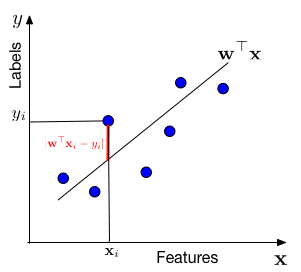
\includegraphics[scale=0.4]{linreg}
\end{figure}
\end{frame}

\section{Extensions}
%------------------------------------------------
\subsection{Simple and multiple linear regression}
\begin{frame}
\frametitle{Simple and multiple linear regression}
\begin{block}{Simple and multiple linear regression}
	The very simplest case of a single scalar predictor variable x and a single scalar response variable y is known as simple linear regression. The extension to multiple and/or vector-valued predictor variables (denoted with a capital X) is known as multiple linear regression, also known as multivariable linear regression. Nearly all real-world regression models involve multiple predictors, and basic descriptions of linear regression are often phrased in terms of the multiple regression model.
\end{block}
\begin{figure}[h]
    \centering
    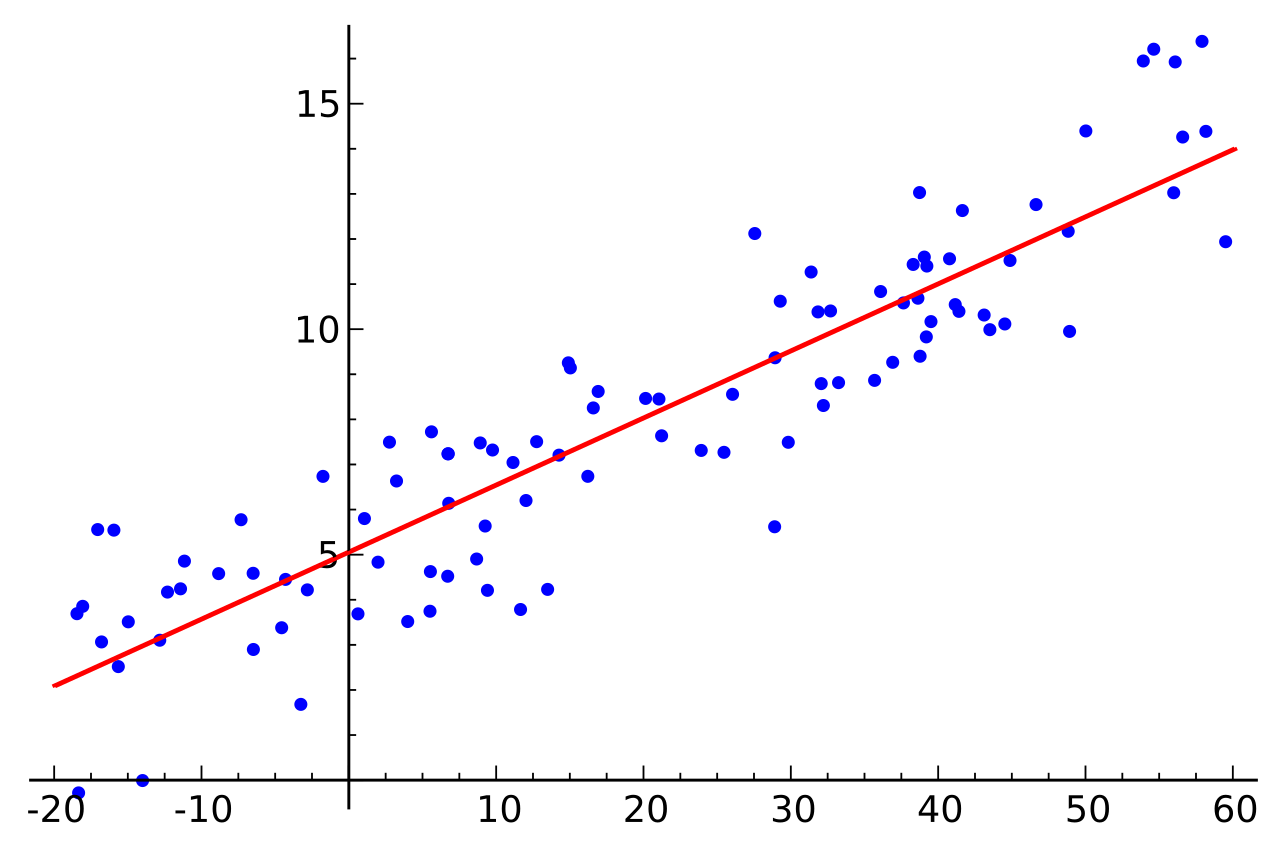
\includegraphics[scale=0.1]{1280px-Linear_regression}
\end{figure}
\end{frame}

\subsection{Generalized linear models}
\begin{frame}
\frametitle{Generalized linear models}
\begin{block}{Generalized linear models}
	Generalized linear models (GLMs) are a framework for modeling response variables that are bounded or discrete. This is used, for example:
\end{block}
\begin{itemize}
\item \small when modeling positive quantities (e.g. prices or populations) that vary over a large scale��which are better described using a skewed distribution such as the log-normal distribution or Poisson distribution (although GLMs are not used for log-normal data, instead the response variable is simply transformed using the logarithm function);
\item \small when modeling categorical data, such as the choice of a given candidate in an election (which is better described using a Bernoulli distribution/binomial distribution for binary choices, or a categorical distribution/multinomial distribution for multi-way choices), where there are a fixed number of choices that cannot be meaningfully ordered;
\item \small when modeling ordinal data, e.g. ratings on a scale from 0 to 5, where the different outcomes can be ordered but where the quantity itself may not have any absolute meaning (e.g. a rating of 4 may not be "twice as good" in any objective sense as a rating of 2, but simply indicates that it is better than 2 or 3 but not as good as 5).	
\end{itemize}
\end{frame}

\subsection{Hierarchical linear models}
\begin{frame}
\frametitle{Hierarchical linear models}
\begin{block}{Hierarchical linear models}
	Hierarchical linear models (or multilevel regression) organizes the data into a hierarchy of regressions, for example where A is regressed on B, and B is regressed on C. It is often used where the variables of interest have a natural hierarchical structure such as in educational statistics, where students are nested in classrooms, classrooms are nested in schools, and schools are nested in some administrative grouping, such as a school district. The response variable might be a measure of student achievement such as a test score, and different covariates would be collected at the classroom, school, and school district levels.
\end{block}
\end{frame}





%------------------------------------------------
\section{Estimating with MLE}
%------------------------------------------------
\subsection{Estimating with MLE}
\begin{frame}
\frametitle{Estimating with MLE}
\begin{math}
\begin{aligned}
\mathbf{w} &= \operatorname*{argmax}_{\mathbf{\mathbf{w}}} P(y_1,\mathbf{x}_1,...,y_n,\mathbf{x}_n|\mathbf{w})\\
&= \operatorname*{argmax}_{\mathbf{\mathbf{w}}} \prod_{i=1}^n P(y_i,\mathbf{x}_i|\mathbf{w})\\
&= \operatorname*{argmax}_{\mathbf{\mathbf{w}}} \prod_{i=1}^n P(y_i|\mathbf{x}_i,\mathbf{w})P(\mathbf{x}_i|\mathbf{w})\\
&= \operatorname*{argmax}_{\mathbf{\mathbf{w}}} \prod_{i=1}^n P(y_i|\mathbf{x}_i,\mathbf{w})P(\mathbf{x}_i)\\
&= \operatorname*{argmax}_{\mathbf{\mathbf{w}}} \prod_{i=1}^n P(y_i|\mathbf{x}_i,\mathbf{w})\\
&= \operatorname*{argmax}_{\mathbf{\mathbf{w}}} \sum_{i=1}^n \log\left[P(y_i|\mathbf{x}_i,\mathbf{w})\right] \\
&= \operatorname*{argmax}_{\mathbf{\mathbf{w}}} \sum_{i=1}^n \left[ \log\left(\frac{1}{\sqrt{2\pi\sigma^2}}\right) + \log\left(e^{-\frac{(\mathbf{x}_i^\top\mathbf{w}-y_i)^2}{2\sigma^2}}\right)\right]\\
\end{aligned}
\end{math}
\end{frame}
%------------------------------------------------
%\subsection{K value}
\begin{frame}
\frametitle{Estimating with MLE}
\begin{math}
\begin{aligned}
&= \operatorname*{argmax}_{\mathbf{\mathbf{w}}} -\frac{1}{2\sigma^2}\sum_{i=1}^n (\mathbf{x}_i^\top\mathbf{w}-y_i)^2\\
&= \operatorname*{argmin}_{\mathbf{\mathbf{w}}} \frac{1}{n}\sum_{i=1}^n (\mathbf{x}_i^\top\mathbf{w}-y_i)^2\\
\vspace{1cm}
\end{aligned}
\end{math}
\begin{itemize}
\item We are minimizing a loss function, $l(\mathbf{w}) = \frac{1}{n}\sum_{i=1}^n (\mathbf{x}_i^\top\mathbf{w}-y_i)^2$. This particular loss function is also known as the squared loss or Ordinary Least Squares (OLS). OLS can be optimized with gradient descent, Newton's method, or in closed form.
Closed Form: $\mathbf{w} = (\mathbf{X X^\top})^{-1}\mathbf{X}\mathbf{y}^\top$ where $\mathbf{X}=\left[\mathbf{x}_1,\dots,\mathbf{x}_n\right]$ and $\mathbf{y}=\left[y_1,\dots,y_n\right]$.	
\end{itemize}
\end{frame}
%%------------------------------------------------


%%------------------------------------------------
\section{Estimating with MAP}
%------------------------------------------------
\subsection{Estimating with MAP}
\begin{frame}
\frametitle{Estimating with MAP}

 Additional Model Assumption:$P(\mathbf{w}) = \frac{1}{\sqrt{2\pi\tau^2}}e^{-\frac{\mathbf{w}^\top\mathbf{w}}{2\tau^2}}$

%Additional Model Assumption:
\begin{math}
\begin{aligned}
%$P(\mathbf{w}) = \frac{1}{\sqrt{2\pi\tau^2}}e^{-\frac{\mathbf{w}^\top\mathbf{w}}{2\tau^2}}$
\mathbf{w} &= \operatorname*{argmax}_{\mathbf{\mathbf{w}}} P(\mathbf{w}|y_1,\mathbf{x}_1,...,y_n,\mathbf{x}_n)\\
&= \operatorname*{argmax}_{\mathbf{\mathbf{w}}} \frac{P(y_1,\mathbf{x}_1,...,y_n,\mathbf{x}_n|\mathbf{w})P(\mathbf{w})}{P(y_1,\mathbf{x}_1,...,y_n,\mathbf{x}_n)}\\
&= \operatorname*{argmax}_{\mathbf{\mathbf{w}}} P(y_1,\mathbf{x}_1,...,y_n,\mathbf{x}_n|\mathbf{w})P(\mathbf{w})\\
&= \operatorname*{argmax}_{\mathbf{\mathbf{w}}}
\left[\prod_{i=1}^nP(y_i,\mathbf{x}_i|\mathbf{w})\right]P(\mathbf{w})\\
&= \operatorname*{argmax}_{\mathbf{\mathbf{w}}}
\left[\prod_{i=1}^nP(y_i|\mathbf{x}_i,\mathbf{w})P(\mathbf{x}_i|\mathbf{w})\right]P(\mathbf{w})\\
&= \operatorname*{argmax}_{\mathbf{\mathbf{w}}}
\left[\prod_{i=1}^nP(y_i|\mathbf{x}_i,\mathbf{w})P(\mathbf{x}_i)\right]P(\mathbf{w})\\
%&= \operatorname*{argmin}_{\mathbf{\mathbf{w}}} \frac{1}{n} \sum_{i=1}^n (\mathbf{x}_i^\top\mathbf{w}-y_i)^2 + \lambda|| \mathbf{w}||_2^2\tag*{$\lambda=\frac{\sigma^2}{n\tau^2}$}\\
\end{aligned}
\end{math}
\end{frame}

%\subsection{1-nearest neighbor classifier}
\begin{frame}
\frametitle{Estimating with MAP}
%Additional Model Assumption:
\begin{math}
\begin{aligned}
&= \operatorname*{argmax}_{\mathbf{\mathbf{w}}} \left[\prod_{i=1}^n P(y_i|\mathbf{x}_i,\mathbf{w})\right]P(\mathbf{w})\\
&= \operatorname*{argmax}_{\mathbf{\mathbf{w}}} \sum_{i=1}^n  \log P(y_i|\mathbf{x}_i,\mathbf{w})+ \log P(\mathbf{w})\\
&= \operatorname*{argmin}_{\mathbf{\mathbf{w}}} \frac{1}{2\sigma^2} \sum_{i=1}^n (\mathbf{x}_i^\top\mathbf{w}-y_i)^2 + \frac{1}{2\tau^2}\mathbf{w}^\top\mathbf{w}\\
&= \operatorname*{argmin}_{\mathbf{\mathbf{w}}} \frac{1}{n} \sum_{i=1}^n (\mathbf{x}_i^\top\mathbf{w}-y_i)^2 + \lambda|| \mathbf{w}||_2^2 \\
\vspace{1cm}
\end{aligned}
\end{math}
\begin{itemize}
\item This objective is known as Ridge Regression. It has a closed form solution of: $\mathbf{w} = (\mathbf{X X^{\top}}+\lambda \mathbf{I})^{-1}\mathbf{X}\mathbf{y}^\top,$ where $\mathbf{X}=\left[\mathbf{x}_1,\dots,\mathbf{x}_n\right]$ and $\mathbf{y}=\left[y_1,\dots,y_n\right]$.
\end{itemize}
\end{frame}

\section{Applications}
%%------------------------------------------------
%\subsection{Trend line}
%\begin{frame}
%\frametitle{Trend line:}
%\begin{block}{Trend line}
%	A trend line represents a trend, the long-term movement in time series data after other components have been accounted for. It tells whether a particular data set (say GDP, oil %prices or stock prices) have increased or decreased over the period of time. A trend line could simply be drawn by eye through a set of data points, but more properly their %position and slope is calculated using statistical techniques like linear regression. Trend lines typically are straight lines, although some variations use higher degree %polynomials depending on the degree of curvature desired in the line.
%\end{block}
%\end{frame}

\subsection{Finance}
\begin{frame}
\frametitle{Finance}
\begin{block}{Finance}
	The capital asset pricing model uses linear regression as well as the concept of beta for analyzing and quantifying the systematic risk of an investment. This comes directly from the beta coefficient of the linear regression model that relates the return on the investment to the return on all risky assets.
\end{block}
\begin{block}{Economics}
	Linear regression is the predominant empirical tool in economics. For example, it is used to predict consumption spending, fixed investment spending, inventory investment, purchases of a country's exports, spending on imports, the demand to hold liquid assets, labor demand, and labor supply.
\end{block}
\end{frame}

\subsection{Environmental science}
\begin{frame}
\frametitle{Environmental science}
\begin{block}{Environmental science}
	Linear regression finds application in a wide range of environmental science applications. In Canada, the Environmental Effects Monitoring Program uses statistical analyses on fish and benthic surveys to measure the effects of pulp mill or metal mine effluent on the aquatic ecosystem.
\end{block}
\begin{block}{Machine learning}
	Linear regression plays an important role in the field of artificial intelligence such as machine learning. The linear regression algorithm is one of the fundamental supervised machine-learning algorithms due to its relative simplicity and well-known properties.
\end{block}
\end{frame}


\section{Summary}
%------------------------------------------------
\subsection{Summary}
\begin{frame}
\frametitle{Summary}
\begin{itemize}
	\item \textbf{Ordinary Least Squares}:\\
    $\operatorname*{min}_{\mathbf{\mathbf{w}}} \frac{1}{n}\sum_{i=1}^n (\mathbf{x}_i^\top\mathbf{w}-y_i)^2$\\
    Squared loss\\
    No regularization\\
    Closed form: $\mathbf{w} = (\mathbf{X X^\top})^{-1}\mathbf{X} \mathbf{y}^\top$\\
    \item \textbf{Ridge Regression}:\\
    $\operatorname*{min}_{\mathbf{\mathbf{w}}} \frac{1}{n}\sum_{i=1}^n (\mathbf{x}_i^\top\mathbf{w}-y_i)^2 + \lambda ||\mathbf{w}||_2^2$\\
    Squared loss \\
    $l2\text{-regularization}$\\
    Closed form: $\mathbf{w} = (\mathbf{X X^{\top}}+\lambda \mathbf{I})^{-1}\mathbf{X} \mathbf{y}^\top$
\end{itemize}
\end{frame}

%------------------------------------------------
\subsection{Code eamples}
\begin{frame}
\frametitle{Simple linear regression implementation}
\href{https://github.com/IEC-lab/MachineLearning2019/blob/master/Linear Regression/linear_regression.py}{Simple linear regression implementation code click here}
\end{frame}

\begin{frame}
\frametitle{housing price prediction}
\href{https://github.com/IEC-lab/MachineLearning2019/blob/master/Linear Regression/houseprice.py}{housing price prediction code click here}
\end{frame}
%%------------------------------------------------

%%------------------------------------------------
%\section{Reference}
%------------------------------------------------
%\begin{frame}
%\frametitle{Reference}
%\begin{thebibliography}{4}
%\bibitem{LS-SPH} F. Zou, C. Liu, H. Ling, H. Feng, L. Yan, and D. Li, "Least square regularized spectral hashing for similarity search," Signal Processing, vol. 93, pp. 2265-2273, 2013. (SCI,EI)
%\bibitem{KMFH} F. Zou, Y. Chen, J. Song, K. Zhou, Y. Yang, and N. Sebe, "Compact image fingerprint via multiple kernel hashing," IEEE Transactions on Multimedia, vol. 17, pp. 1006-1018, 2015. (SCI,EI)
%\bibitem{KNPH} C. Liu, H. Ling, F. Zou, L. Yan, Y. Wang, H. Feng, et al., "Kernelized neighborhood preserving hashing for social-network-oriented digital fingerprints," IEEE Transactions on Information Forensics and Security, vol. 9, pp. 2232-2247, 2014. (SCI,EI)
%\bibitem{DTSH} Liu, Yu; Song, Jingkuan; Zhou, Ke; Yan, Lingyu; Liu, Li; Zou, Fuhao; Shao, Ling, "Deep Self-taught Hashing for Image Retrieval," IEEE Transactions on Cybernetics, May 3, 2018. (SCI,EI)
%\bibitem{DeepFace} Fuhao Zou, Fan Yang, Wei Chen,Kai Lia, Jingkuan Song, Jingcai Chen, Hefei Ling, "Fast Large Scale Deep Face Search," Pattern Recognition Letters, Januray 3, 2019. (SCI,EI)
%\end{thebibliography}
%\end{frame}
%------------------------------------------------
\begin{frame}
\Huge{\centerline{The End}}
\end{frame}

\end{CJK*}
\end{document}
 
